\documentclass[12pt]{article}
% Préambule commun à tous les documents extraits de « La Revue CAPES »
\usepackage[T1]{fontenc}
\usepackage[utf8]{inputenc}
\usepackage{lmodern}
\usepackage{amsmath,amssymb,amsthm,amsfonts,mathrsfs}
\usepackage{setspace}
\usepackage{listings}
\usepackage{pgfplots}
\pgfplotsset{compat=1.18}
\usepackage{longtable}
\usepackage{adjustbox}
\usepackage{lettrine}
\usepackage{tkz-tab}
\usepackage{changepage}
\usepackage{pdflscape}
\usepackage{graphicx}
\usepackage{tikz}
\usepackage{xcolor}
\usepackage[a4paper,top=2cm,bottom=2.5cm,left=2.5cm,right=2cm]{geometry}
\usepackage{fancyhdr}
\usepackage{draftwatermark}
\SetWatermarkText{La RevueCapes}
\SetWatermarkLightness{0.9}
\SetWatermarkScale{2}
\usepackage{hyperref}
\hypersetup{colorlinks=true,linkcolor=blue!50!black,urlcolor=blue!50!black}

\definecolor{revue}{RGB}{20,60,120}

\pagestyle{fancy}
\fancyhf{}
\renewcommand{\headrulewidth}{0.4pt}
\setlength{\headheight}{15pt}

% \entete{Matière}{Titre}{Type de document}
\newcommand{\entete}[3]{%
  \fancyhead[L]{\small\textsc{La Revue CAPES} -- #1}%
  \fancyhead[R]{\small #2}%
  \fancyfoot[C]{\thepage}%
  \thispagestyle{plain}%
  \begin{center}
    {\color{revue}\rule{\textwidth}{1.2pt}}\\[4pt]
    {\small\textsc{Concours directs CAP-CEG / CAPES -- Burkina Faso}}\\[6pt]
    {\LARGE\bfseries\color{revue} #2}\\[6pt]
    {\large\itshape #1 -- #3}\\[2pt]
    {\color{revue}\rule{\textwidth}{1.2pt}}
  \end{center}
  \vspace{0.5cm}%
}

% Encadré pour les remarques ajoutées dans les corrigés
\newcommand{\remarque}[1]{\par\medskip\noindent\fcolorbox{revue}{revue!6}{\parbox{\dimexpr\linewidth-2\fboxsep-2\fboxrule}{\textbf{\color{revue}Remarque.} #1}}\par\medskip}


\begin{document}
\entete{Mathématiques}{Corrigé détaillé -- Session 2019}{Correction}
\begin{spacing}{1.5}

\textbf{Exercice 1}

On considère la matrice carrée d'ordre 3 définie par  : 

$M=\begin{pmatrix}
11 & -5 & 5 \\ 
-5 & 3 & -3 \\ 
5 & -3 & 3
\end{pmatrix}$

1. Déterminons le polynôme caractéristique de $M$, ainsi que son spectre.

\begin{align*}
P_M(x)=\det(M-xI_3)&=\begin{vmatrix}
11-x & -5 & 5 \\ 
-5 & 3-x & -3 \\ 
5 & -3 & 3-x
\end{vmatrix}\leftarrow c_3+c_2\\
&=\begin{vmatrix}
11-x & -5 & 0 \\ 
-5 & 3-x & -x \\ 
5 & -3 & -x
\end{vmatrix}\leftarrow L_2-L_3\\
&=x\begin{vmatrix}
11-x & -5 & 0 \\ 
-10 & 6-x & 0 \\ 
5 & -3 & -1
\end{vmatrix}\\
&=-x\begin{vmatrix}
11-x & -5 \\
-10 & 6-x 
\end{vmatrix}\\
&=-x((11-x)(6-x)-50)\\
&=-x(66-11x-6x+x^2-50)\\
&=-x(x^2-17x+16)\\
\end{align*}

Factorisation de $x^2-17x+16$

$\Delta=225=(15)^2$

$x=\frac{17-15}{2}=1$ ou $x=\frac{17+15}{2}=16$

Donc $P_M(x)=-x(x-1)(x-16)$.

Ainsi spectre de $M$ est $Sp(M)=\{0;1;16\}$

2. Les sous espaces propres associés aux différentes valeurs propres.

Soit $E_\lambda$ le sous-espace propre lié à la valeur propre $\lambda$

\[
E_\lambda=\{u=(x,y,z)\in \mathbb{R}^3/Mu=\lambda u\}
\]

\medskip
$\bullet$ Pour $\lambda=0$, on a :

$\forall u\in E_0,Mu=0\Rightarrow \begin{pmatrix}
11 & -5 & 5 \\ 
-5 & 3 & -3 \\ 
5 & -3 & 3
\end{pmatrix}\begin{pmatrix}
x\\
y\\
z
\end{pmatrix}=\begin{pmatrix}
0\\
0\\
0
\end{pmatrix}\Rightarrow \begin{cases}
11x-5y+5z=0\\
-5x+3y-3z=0\\
5x-3y+3z=0
\end{cases}\Rightarrow \begin{cases}
11x-5y+5z=0(1)\\
5x-3y+3z=0(2)
\end{cases}$

$(2)\Longrightarrow x=\frac{3}{5}(y-z)$

$(1)\Longrightarrow \frac{33}{5}(y-z)-5y+5z=0\Longrightarrow  \frac{8}{5}y-\frac{8}{5}=0\Longrightarrow y-z=0\Longrightarrow y=z$ $\Rightarrow x=0$

$\Rightarrow u=\begin{pmatrix}
0\\
y\\
y
\end{pmatrix}=y\begin{pmatrix}
0\\
1  \\
1
\end{pmatrix}\Rightarrow E_0=\langle \begin{pmatrix}
0\\
1\\
1
\end{pmatrix}\rangle$

$\bullet$ Pour $\lambda=1$, on a :

$\begin{pmatrix}
11 & -5 & 5 \\ 
-5 & 3 & -3 \\ 
5 & -3 & 3
\end{pmatrix}\begin{pmatrix}
x\\
y\\
z
\end{pmatrix}=\begin{pmatrix}
x\\
y\\
z
\end{pmatrix}=\begin{cases}
10x-5y+5z=0(1)\\
-5x+2y-3z=0(2)\\
5x-3y+2z=0(3)
\end{cases}$

$(2)+(3)\Rightarrow z=-y (4)$

$(4)$ dans $(1)\Longrightarrow x=y$

$\Rightarrow u=\begin{pmatrix}
y\\
y\\
-y
\end{pmatrix}=y\begin{pmatrix}
1\\
1\\
-1
\end{pmatrix}\Rightarrow E_{1}=\langle \begin{pmatrix}
1 \\
1 \\
-1
\end{pmatrix}\rangle$

$\bullet$ Pour $\lambda=16$, on a :

$\begin{pmatrix}
11 & -5 & 5 \\ 
-5 & 3 & -3 \\ 
5 & -3 & 3
\end{pmatrix}\begin{pmatrix}
x\\
y\\
z
\end{pmatrix}=16\begin{pmatrix}
x\\
y\\
z
\end{pmatrix}=\begin{cases}
-5x-5y+5z=0(1)\\
-5x-13y-3z=0(2)\\
5x-3y-13z=0(3)
\end{cases}$

$(2)+(3)\Rightarrow z=-y (4)$

$(4)$ dans $(1)\Longrightarrow x=-2y$

$\Rightarrow u=\begin{pmatrix}
-2y\\
y\\
-y
\end{pmatrix}=-y\begin{pmatrix}
2\\
-1\\
1
\end{pmatrix}\Rightarrow E_{16}=\langle \begin{pmatrix}
2 \\
-1 \\
1
\end{pmatrix}\rangle$


3. $M$ est diagonalisable car le polynôme caractéristique de $M$ est scindé en racines simples. Ou autrement car les valeurs propres sont distinctes deux à deux.

\medskip
\textbf{Diagonalisons $M$}

On a la base $B=\langle \begin{pmatrix}
0\\
1\\
1
\end{pmatrix},\begin{pmatrix}
1 \\
1 \\
-1
\end{pmatrix},\begin{pmatrix}
2 \\
-1 \\
1
\end{pmatrix}\rangle$.

Dans la base $B$, $D=\begin{pmatrix}
0 & 0 & 0 \\ 
0 & 1 & 0 \\ 
0 & 0 & 16
\end{pmatrix}$ et $P= \begin{pmatrix}
0 & 1  & 2 \\ 
1 & 1  & -1\\ 
1 & -1 & 1 
\end{pmatrix}$

$M=PDP^{-1}$

\medskip
Calculons $P^{-1}$

$P^{-1}=\frac{1}{det(P)}t_{com(P)}$

$det(P)=\begin{vmatrix}
0 & 1  & 2 \\ 
1 & 1  & -1\\ 
1 & -1 & 1 
\end{vmatrix}=-(1+2)+(-1-2)=-6$

$com(P)=\begin{pmatrix}
0 & -2  & -2 \\ 
-3 & -2  & 1\\ 
-3 & 2 & -1 
\end{pmatrix}\Rightarrow t_{com(P)}=\begin{pmatrix}
0 & -3  & -3 \\ 
-2 & -2  & 2\\ 
-2 & 1 & -1 
\end{pmatrix}$

Ainsi $P^{-1}=-\frac{1}{6}\begin{pmatrix}
0 & -3  & -3 \\ 
-2 & -2  & 2\\ 
-2 & 1 & -1 
\end{pmatrix}=\frac{1}{6}\begin{pmatrix}
0 & 3  & 3 \\ 
2 & 2  & -2\\ 
2 & -1 & 1 
\end{pmatrix}$


4. Déduisons $M^{n}$ $\forall n\in \mathbb{N}$.

$M=PDP^{-1}\Rightarrow M^n=PD^nP^{-1}$ avec $D^n=\begin{pmatrix}
0 & 0 & 0 \\ 
0 & 1 & 0 \\ 
0 & 0 & 16^n
\end{pmatrix}$

$M^n=\frac{1}{6}\begin{pmatrix}
0 & 1  & 2 \\ 
1 & 1  & -1\\ 
1 & -1 & 1 
\end{pmatrix}\begin{pmatrix}
0 & 0 & 0 \\ 
0 & 1 & 0 \\ 
0 & 0 & 16^n
\end{pmatrix}\begin{pmatrix}
0 & 3  & 3 \\ 
2 & 2  & -2\\ 
2 & -1 & 1 
\end{pmatrix}$

$M^n=\frac{1}{6}\begin{pmatrix}
2+4.(16)^n & 2-2.(16)^n  & -2+2.(16)^n \\ 
2-2.(16)^n & 2+(16)^n  & -2-(16)^n\\ 
-2+2.(16)^n & -2-(16)^n & 2+(16)^n 
\end{pmatrix}$ $\forall n\in \mathbb{N}$

\medskip
\medskip
\textbf{Exercice 2}

On considère la fonction $2\pi$ périodique impaire définie par : 

$h(x)=x(\pi-x); \forall {x}\in [0,\pi]$.

1. Représentons graphiquement cette fonction sur $[-2\pi,2\pi]$.

\underline{\textbf{ Étude de $h$}}

$h$ est périodique de période $2\pi$, alors son domaine d'étude peut être réduit à $[-\pi,\pi]$. De plus, $h$ est impaire, c'est-à-dire $h(-x)=-h(x)$, donc $h$ est symétrique par rapport à l'axe des ordonnées. Ainsi le domaine d'étude peut être réduit à $[0,\pi]$. Nous pouvons tracer $h$ sur $[0,\pi]$ et utiliser la périodicité pour étendre le graphique. Sur l'intervalle $[0, \pi]$, la fonction est donnée par $h(x) = x(\pi - x)$.

$h$ est un polynôme, donc continue et dérivable sur $[0,\pi]$

et $h'(x)=\pi-2x$

Soit $h'(x)=0\Rightarrow \pi-2x=0\Rightarrow x=\frac{\pi}{2}$

-Si $x\in [0,\frac{\pi}{2}]$, $h'(x)\geq 0$, alors $h$ est croissante.

-Si $x\in [\frac{\pi}{2},\pi]$, $h'(x)\leq 0$, alors $h$ est décroissante.

\medskip
\underline{Tableau de variation sur $[0,\pi]$}

$h(0)=0$, $h(\frac{\pi}{2})=\frac{\pi^2}{4}$, $h(0)=0$

\begin{center}
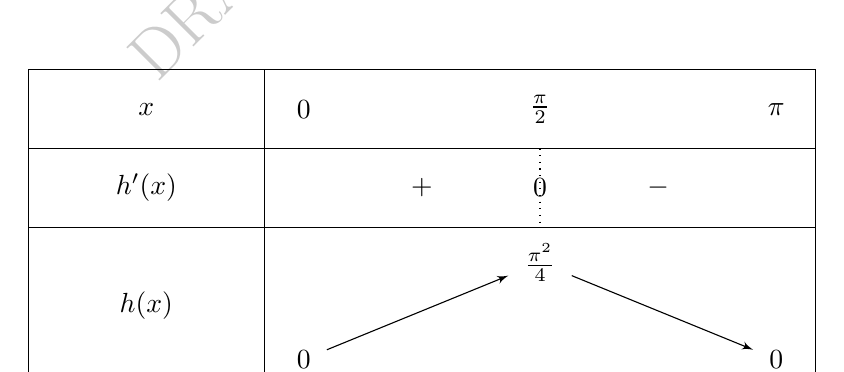
\begin{tikzpicture} 
\tkzTabInit[lgt=3, espcl=3]{$x$ /1, $h'(x)$ /1, $h(x)$ /2}{$0$, $\frac{\pi}{2}$, $\pi$} 
\tkzTabLine{, +, z, -,} 
\tkzTabVar{-/ $0$, +/ $\frac{\pi^2}{4}$ , -/ $0$}
\end{tikzpicture} 
\end{center}

\medskip
\underline{Graphe de $h$}
 
 
 

 


2) Calcul des coefficients de Fourier

La fonction \( h(x) = x(\pi - x) \) est impaire et \( 2\pi \)-périodique. Comme elle est impaire, tous les coefficients \( a_n \) (cosinus) sont nuls. On calcule uniquement les coefficients \( b_n \) (sinus) :

\[
b_n = \frac{2}{\pi} \int_0^\pi h(x) \sin(nx) \, dx.
\]

En remplaçant \( h(x) = x(\pi - x) \), on a :

\[
b_n = \frac{2}{\pi} \int_0^\pi x(\pi - x) \sin(nx) \, dx.
\]

On décompose l'intégrale :

\[
b_n = \frac{2}{\pi} \left( \pi \int_0^\pi x \sin(nx) \, dx - \int_0^\pi x^2 \sin(nx) \, dx \right).
\]

\textbf{Calcul des intégrales}

Première intégrale

\[
\int_0^\pi x \sin(nx) \, dx = \left[ -\frac{x \cos(nx)}{n} \right]_0^\pi + \frac{1}{n} \int_0^\pi \cos(nx) \, dx = \frac{(-1)^{n+1} \pi}{n}.
\]

Deuxième intégrale

\[
\int_0^\pi x^2 \sin(nx) \, dx = \left[ -\frac{x^2 \cos(nx)}{n} \right]_0^\pi + \frac{2}{n} \int_0^\pi x \cos(nx) \, dx.
\]

En utilisant le résultat de la première intégrale, on trouve :

\[
\int_0^\pi x^2 \sin(nx) \, dx = \frac{(-1)^{n+1} \pi^2}{n} + \frac{2}{n} \cdot \frac{(-1)^n - 1}{n^2}.
\]

\textbf{Combinaison des résultats}

En combinant les résultats, on obtient :

\[
b_n = \frac{2}{\pi} \left( \pi \cdot \frac{(-1)^{n+1} \pi}{n} - \left( \frac{(-1)^{n+1} \pi^2}{n} + \frac{2((-1)^n - 1)}{n^3} \right) \right).
\]

Après simplification, on trouve :

\[
b_n = \frac{4((-1)^n - 1)}{\pi n^3}.
\]


3) Développement en série de Fourier

Le développement en série de Fourier de \( h(x) \) est :

\[
h(x) = \sum_{n=1}^\infty b_n \sin(nx),
\]

avec \( b_n = \frac{4((-1)^n - 1)}{\pi n^3} \). On peut écrire :

\[
h(x) = \sum_{n=1}^\infty \frac{4((-1)^n - 1)}{\pi n^3} \sin(nx).
\]

4) Calcul des sommes \( S_1 \) et \( S_2 \)

\textbf{Calcul de \( S_1 = \sum_{n=0}^\infty \frac{(-1)^n}{(2n+1)^3} \)}

On utilise le développement en série de Fourier de \( h(x) \) en \( x = \frac{\pi}{2} \). On a :

\[
h\left(\frac{\pi}{2}\right) = \frac{\pi}{2} \left(\pi - \frac{\pi}{2}\right) = \frac{\pi^2}{4}.
\]

D'autre part, en évaluant la série de Fourier en \( x = \frac{\pi}{2} \), on obtient :

\[
h\left(\frac{\pi}{2}\right) = \sum_{n=1}^\infty b_n \sin\left(n \cdot \frac{\pi}{2}\right).
\]

Comme \( \sin\left(n \cdot \frac{\pi}{2}\right) \) vaut \( 0 \) pour \( n \) pair et \( (-1)^k \) pour \( n = 2k + 1 \), on a :

\[
\frac{\pi^2}{4} = \sum_{k=0}^\infty b_{2k+1} (-1)^k.
\]

En remplaçant \( b_{2k+1} \), on trouve :

\[
\frac{\pi^2}{4} = \sum_{k=0}^\infty \frac{4((-1)^{2k+1} - 1)}{\pi (2k+1)^3} (-1)^k.
\]

Simplification :

\[
\frac{\pi^2}{4} = \sum_{k=0}^\infty \frac{4(-2)}{\pi (2k+1)^3} (-1)^k = -\frac{8}{\pi} \sum_{k=0}^\infty \frac{(-1)^k}{(2k+1)^3}.
\]

On en déduit :

\[
S_1 = \sum_{k=0}^\infty \frac{(-1)^k}{(2k+1)^3} = -\frac{\pi^3}{32}.
\]

\textbf{Calcul de \( S_2 = \sum_{n=0}^\infty \frac{1}{(2n+1)^6} \)}

On utilise l'identité de Parseval pour la série de Fourier de \( h(x) \). L'identité de Parseval donne :

\[
\frac{1}{\pi} \int_{-\pi}^\pi h(x)^2 \, dx = \sum_{n=1}^\infty b_n^2.
\]

Comme \( h(x) \) est impaire, on a :

\[
\int_{-\pi}^\pi h(x)^2 \, dx = 2 \int_0^\pi h(x)^2 \, dx.
\]

Calcul de \( \int_0^\pi h(x)^2 \, dx \) :

\[
\int_0^\pi x^2 (\pi - x)^2 \, dx = \int_0^\pi x^2 (\pi^2 - 2\pi x + x^2) \, dx = \pi^2 \int_0^\pi x^2 \, dx - 2\pi \int_0^\pi x^3 \, dx + \int_0^\pi x^4 \, dx.
\]

En calculant chaque intégrale, on trouve :

\[
\int_0^\pi h(x)^2 \, dx = \frac{\pi^5}{30}.
\]

Ainsi, l'identité de Parseval donne :

\[
\frac{1}{\pi} \cdot 2 \cdot \frac{\pi^5}{30} = \sum_{n=1}^\infty b_n^2.
\]

Simplification :

\[
\frac{\pi^4}{15} = \sum_{n=1}^\infty \left( \frac{4((-1)^n - 1)}{\pi n^3} \right)^2 = \frac{16}{\pi^2} \sum_{n=1}^\infty \frac{((-1)^n - 1)^2}{n^6}.
\]

Comme \( ((-1)^n - 1)^2 = 4 \) pour \( n \) impair et \( 0 \) pour \( n \) pair, on a :

\[
\frac{\pi^4}{15} = \frac{16}{\pi^2} \cdot 4 \sum_{k=0}^\infty \frac{1}{(2k+1)^6}.
\]

On en déduit :

\[
S_2 = \sum_{k=0}^\infty \frac{1}{(2k+1)^6} = \frac{\pi^6}{960}.
\]






\medskip\textbf{Exercice 3}


\medskip

\end{spacing}
\end{document}
